\documentclass[12pt,a4paper]{report}
\usepackage{geometry}
\geometry{top=14mm, bottom=15mm}
\usepackage[english]{babel}
\usepackage[utf8]{inputenc}
\usepackage{fancyhdr}
\usepackage{csquotes}
\usepackage{listings}
\usepackage{hyperref}
\usepackage{graphics, graphicx}
\usepackage{graphics, graphicx}
\pagestyle{fancy}
\fancyhf{}
%\rhead{}
%\lhead{}
\fancyfoot[LE,LO]{Data Analytics}
\fancyfoot[RE,RO]{Mini Project - 1}
\renewcommand{\footrulewidth}{1pt}
 \medskip
 \author{Abhijeet Singh Panwar (ID : 201351005)}
\title{Data Analytics\\ Mini Project - 2}

\date{\parbox{\linewidth}{\centering%
  \today\endgraf\bigskip
  Instructor : \endgraf\medskip
  Prof. Bhargab Chattopadhyay\endgraf\bigskip
  Indian Institute of Information Technology, Vadodara}}
\begin{document}
\maketitle
\newpage
\section{Use R to make a map of Gujarat using an R package showing district-wise characteristic}

Solution $\rightarrow$ Given spatial data, in this case \enquote{District-wise Population Density}, it can be incorporated with R map-plotting libraries to generate graphical representation of data, which is more easy to understand and gives a clear idea about the data.
\\

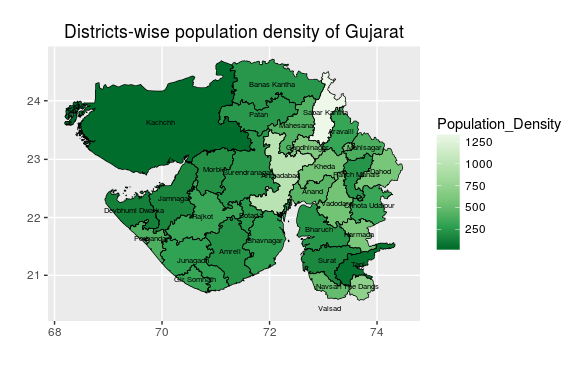
\includegraphics[scale=1]{q1.png}


\textbf{References}
\begin{itemize}
\item \url{http://censusindia.gov.in/2011-prov-results/data_files/gujarat/statement-1.xls}
\item \url{https://en.wikipedia.org/wiki/List_of_districts_of_Gujarat}
\end{itemize}

\textit{Some data is not available in $1^{st}$ reference.}

\section{Mixture models form one of the most fundamental classes of generative models for
clustered data.}
\textbf{For example, run times on unix servers in 100 universities. The following are run times
in seconds.}\\\\
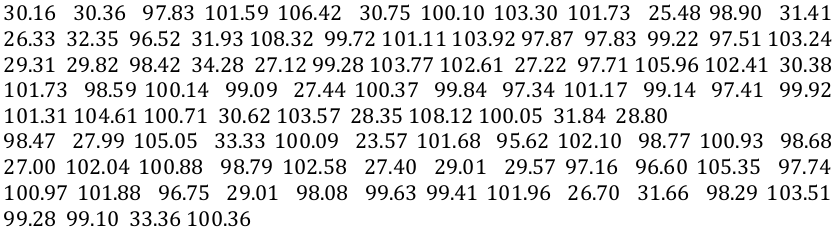
\includegraphics[scale=0.45]{a.png}
\\
\\
Using mixture normal distribution (a bimodal distribution)\\\\
0.7*N$\lbrace \mu_1,{\sigma_1}^2\rbrace$+0.3*N$\lbrace \mu_2,{\sigma_2}^2 \rbrace$\\\\
\textbf{A. Find the maximum likelihood estimates of the unknown parameters and their standard errors.}
\\\\
The basic idea of maximum likelihood is to minimize the negative log likelihood inorder to fit the function to the given data, by tweaking the values of parameters, which in this case are, \textit{$\mu_1,{\sigma_1}^2,\mu_2,{\sigma_2}^2$}.
\\\\
\textbf{Output:}\\
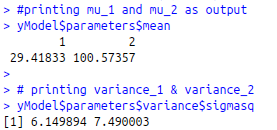
\includegraphics[scale=0.75]{q2_a.png}
\\\\
\textbf{B. Draw a histogram of the data and superimpose the density of the above mixture normal distribution using maximum likelihood estimates of the unknown parameters.}\\
\textbf{Output:}
\\
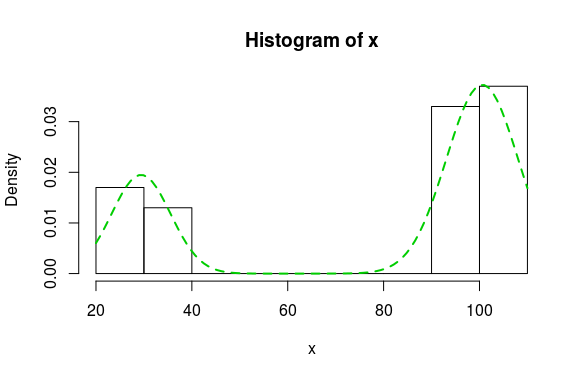
\includegraphics[scale=0.75]{q2_b.png}
\\
\newpage
\section{Appendix}
\textbf{Question 1}\\
\begin{lstlisting}
# R code for Gujrat State
#for Population Density Data:

library(ggplot2)
library(plyr)
library(raster)
library(rgdal)
library(rgeos)
library(sp)

population_density <- read.csv("density.csv", sep = ",")
#fetching map of India from gadm
India <- getData("GADM", country = "India", level = 2)  
Gujarat <- subset(India, NAME_1 == "Gujarat")
#converting map of gujarat into a data matrix
map <- fortify(Gujarat);  
#casting value of id in map into integer and modifying map
map$id <- as.integer(map$id);  
dat <- data.frame(id = 133:165, district = Gujarat@data$NAME_2);	  
#joining gujarat map dataframe with the provided population density data
map_df <- join(map, population_density, by ="id", type="inner")
centers <- data.frame(gCentroid(Gujarat, byid = TRUE));  
centers$state <- dat$district;  	

#plotting the map
ggplot() +
  #creating map having logitude on x-axis & latitude on y-axis, 
  #filled with populaiton density data
  geom_polygon(data = map_df, aes(x = long, y = lat, group = group,
                                  fill = Population_Density)) +
  geom_polygon(data = map_df, aes(x = long, y = lat, group = group),
               fill = NA, color = "black", size = 0.25) +
  scale_fill_distiller(palette = "Greens")+
  geom_text(data = centers, aes(label = state, x = x, y = y), size = 2) + 
  coord_map() + labs(x = "", y = "", title = 
  "Districts-wise population density of Gujarat") 


\end{lstlisting}
\textbf{Question 2}
\\
\\
\textbf{Part A}
\begin{lstlisting}
library(mclust)
#library used to fit a function to a data

x = c(30.16, 30.36, 97.83, 101.59, 106.42, 30.75, 100.10, 103.30, 
101.73, 25.48, 98.90, 31.41, 26.33, 32.35, 96.52, 31.93, 108.32, 
99.72, 101.11, 103.92, 97.87, 97.83, 99.22, 97.51, 103.24, 29.31, 
29.82, 98.42, 34.28, 27.12, 99.28, 103.77, 102.61, 27.22, 97.71, 
105.96, 102.41, 30.38, 101.73, 98.59, 100.14, 99.09, 27.44, 100.37, 
99.84, 97.34, 101.17, 99.14, 97.41, 99.92, 101.31, 104.61, 100.71, 
30.62, 103.57, 28.35, 108.12, 100.05, 31.84, 28.80, 98.47, 27.99, 
105.05, 33.33, 100.09, 23.57, 101.68, 95.62, 102.10, 98.77, 100.93, 
98.68, 27.00, 102.04, 100.88, 98.79, 102.58, 27.40, 29.01, 29.57, 
97.16, 96.60, 105.35, 97.74, 100.97, 101.88, 96.75, 29.01, 98.08, 
99.63, 99.41, 101.96, 26.70, 31.66, 98.29, 103.51, 99.28, 99.10, 
33.36, 100.36)

#BIC for parameterized Gaussian mixture models 
#fitted by EM algorithm initialized by model-based
#hierarchical clustering.
#Here V indicates that data is univariate

BIC = mclustBIC(x, modelNames="V")

#Determines the best model via 
#mclustBIC for a given set of model parameterizations
#and numbers of components

Model = mclustModel(x, yBIC)
#printing mu_1 and mu_2 as output
Model$parameters$mean

# printing variance_1 & variance_2
Model$parameters$variance$sigmasq
\end{lstlisting}
\textbf{Part B}
\begin{lstlisting}
#add two more lines written below to above code

hist(x,prob=TRUE)
curve(0.3*dnorm(x,29.41,6.14)+0.7*dnorm(x,100.57,7.49), 
col=3, lty=2,lwd=2, add=TRUE)
\end{lstlisting}
\end{document}